
\section{Opportunities and Motivation}

There is an abundance of information available from Twitter. Twitter can allow users to post, publish, share and communicate by tweets, which is a 140 characters limited short message. Because of this characters limited feature, the languages in tweets is including a lot of abbreviations and emotion icons. Another important feature is that tweets allow users to use ``@" for reply to specific another users and ``\#" for the self-tagging and self-categories. 

The hashtags in tweets are the words that are preceded by a hash symbol (\#). And there is no space in one hashtag. The hashtags can be used in the beginning, the middle and the end of tweets for the operation of tagging or annotation. In Twitter, if you click the hashtag, it will be linked to the page displaying other tweets that contains the same hashtag on Twitter. Hashtags do not just appear in Twitter. They are also used in Flicker, Pinterest, Instagram, and Facebook. 


Social media users add hashtags in their posts for different goals, including identification label (\#VT or \#Hokie), sentiment label (\#love, \#like, or \#hate), topic label (\#hiking), event label (\#uselection2016) and etc.. Thus, hashtags provide labels for their texts.



Twitter platform is valuable to professional journalists in developing news stories. 

Problem: Twitter information is disorganized, working with it creates high cognitive load and physical demands on users, discover of relevant tweets is difficult because they are not clustered by similarity 

Existing Solutions (How is it done today, second step in Heilmeir, including limits of existing solutions): Existing tools to help organize tweets include Tweet Deck, among others; elaborate on how


Proposed new solution is the tool to organize tweets efficiently. 

The innovation part of my approach is creating hashtags for tweets of similar topic through RNN model. At the same time, our model also bring the tweet embedding into the tweets organizing process.  User can efficiently find similar tweets within vector space of tweets embedding from RNN model. 

Why will it be successful? (performance tests of resulting hashtags from RNN model indicate higher accuracy of hashtags assigned for clustering than other procedures - LDA?)

who cares? what difference will it make?  (journalists should care; your tools should reduce cognitive load, improve discovery of information, etc.

I don’t know about risks and costs or how long it will take Heilmieir steps — these may not be so pertinent for the overview.

What are the mid-term and final ‘exams' to check for success?  These would be the user evaluation studies you should describe in the overview that link back to the steps about why you think your proposed re-design of Tweetdeck will be successful (how will the user evaluation measure this?) and what difference will your re-design make (such as, cognitive and physical loads, news discovery; how will you measure these differences between TweetDeck and your re-design of TweetDeck?).



social media is surging as a new resource for the news discovery and production. 

However, traditional tweets tool, like tweet deck, has a lot of drawbacks.  not good

Users need to organize the tweets better

how to organize tweets better

predict hashtags via RNN: machine learning can help

solution: redesign tweet deck based on rnn model result

for journalist for social media. 

how to design a model. how to design 



organize tweets better for news discovery. design tasks to fit the goal. 

tool did this well, another well, and conclude claims. 


better model will achieve the better user experience.  


\section{Research Questions}

RQ 1:
- Can we use the results from RNN to develop for journalists? 
how to utilize rnn 


- opportunity / motivation

- problem statement

- solution: organize tweets

- existing solution

- however, the failure of existing one

- one orngize is hashtag, but not all have hashtag

- solution to orgnize tweets better with hashtag and embedding
 
- RNN model for hashtag and embedding. 

- solution 



\section{Recurrent Neural Network}
Neural networks is a machine learning approach to map the features of data into an abstract and high-dimensional representation. From 2012, neural network and deep learning models have been successfully applied into different areas of computer vision, speech recognition and natural language processing (NLP) \cite{LeCun2015}. 

Recurrent Neural Network (RNN) is one type of neural network models. RNN model utilizes the sequential information during training process. It processes the same computation for each sequential input, and the output relies on its previous sequential result. In another word, RNN model can be thought as a memory to store the sequential inputs which have been processed earlier.  RNN model has been proved as Turing-complete by Siegelmann et al.\cite{Siegelmann1995} in 1995. It means that just like Turing Machines, any algorithm can be encoded via a RNN model with parameters tuning. 

In NLP research and application area, RNN model has remarkable achievement recently in language modeling (word embedding \cite{Mikolov2013}, sentence embedding \cite{Kiros2015}), machine translation \cite{Sutskever2014}, sentiment analysis \cite{Socher2013}, question answering \cite{Iyyer2014}, and etc.. 

\section{RNN for Hashtag Prediction}

Hashtag can label and classify tweets. It is useful in many scenarios, including tweets search and retrieval \cite{Efron2010}, sentiment analysis \cite{Davidov2010}, and etc.. But, not all the tweets contain hashtag. Based on a survey on a collection of $62,556,331$ tweets, Hong et al. find that there are only about $11\%$ of tweets in their collection contain at least one hashtag \cite{Hong2011a}. So, hashtag prediction for any tweet texts is a necessary task for tweets analysis. 

Hashtag prediction is a multi-class classification task to assign one or several hashtags to the corresponding tweet texts. Hashtag prediction has multiple applications in tweets analysis.  For example, predicted hashtags of tweets would help users to view tweets via different hashtag categories, especially improve the social media journalists to explore tweets efficiently. 

In this thesis, we utilize recurrent neural network (RNN) to train a classification model for hashtag prediction of tweet texts. The model can achieve $51.86\%$ in prediction rate, which is ~2x higher than the traditional Bag-Of-Word (BOW) prediction model.

\section{Hidden States Visual Analytics for RNN}

After training process, RNN models can classify the data in high performance. However, RNN models are black-boxes. Even model creators cannot interpret why their models achieves in high performance. They also do not have hints about what features the model has learned from the data. Thus, except high performance, model creators do not have evidences from model itself to support their decision making.  For example, our RNN hashtag prediction model can achieve $51.86\%$ in prediction rate. But from model itself, we cannot find any evidence to let us understand how the model achieve this high prediction rate. 

Under the hood of RNN models, they have tons of parameters and repeatedly compute non-linear activation functions for large number of their hidden states. Due to these factors, how to interpret and understand RNN model is a challenge work and an active research topic in deep learning area. Few researchers tried to interpret RNN models via studying the changes in hidden states over time \cite{Strobelt2016} \cite{Li2016}, . But they found some interpretable patterns with large noise and interruptions. 

Visual analytics and relevant interaction techniques are potential to aid sensemaking process \cite{Pirolli2005} of RNN models understanding and interpretion. It can support users to find latent patterns of RNN hidden states and reveal them in visual context. However, how to design efficient and usable visual representations of RNN hidden states with necessary interactions to assist sensemaking is still challenging.


\section{Design a UI for news discovery application}

\section{Usability of news discovery application}

\section{Research Questions}

In this thesis, we will explore how to utilize the Recurrent Neural Network (RNN) techniques for tweets analysis, such as hashtag prediction, tweets clustering, and interactive visualization?



In order to state them, two key research questions (RQs) are listed as following: 

\subsection{RQ 1: How to build a Recurrent Neural Network (RNN) based tweets visual analytics system?}

\begin{itemize}
    \item How we can build a RNN model to predict the hashtag of tweets?
    \item How we can build a RNN model to search 
    \item How to design a system to organize tweets with the results from our RNN model? 

\end{itemize}

To answer Research Question 1,  firstly, we utilize recurrent neural network (RNN) to train a classification model for hashtag prediction of any texts. Our RNN model can achieve $51.86\%$ in prediction rate, which is ~2x higher than the traditional Bag-Of-Word (BOW) prediction model. Secondly, we built a RNN we designed a rumor tweets visualization system with the sentence embeddings from our RNN model. Thirdly, we will conduct a user study to find the key design trade off among our RNN model, visualization representations, and interactive strategy.

    
\subsection{RQ 2: How effective are our tweets organization system designed to support sensemaking process of tweets  understanding? }

\begin{itemize}

    \item What is the key design trade off among our RNN model, tweets representations, and interactive strategy?

    \item Would our proposed design visualization in RQ1 be able to help users more effectively gain insights about how the black-box RNN model works? 

    \item How does our proposed RNN hidden states visualization impact users’ understanding and interpretation of RNN model?
    
    \item Can users answer what information a RNN model learns and stores in its hidden states via our design?
    
    \item Can users find the abstract, sentiment information, concepts of inputs with the hidden states pattern in our visualization design?
    
    \item What are the strategies of users to use in our design to find latent patterns and form hypotheses about RNN hidden states?
    
    \item Compare to other RNN visualization approaches\cite{Strobelt2016}, what differences can be observed in the users’ workflow, process, and, insight?
    
    \item Can our design be deployed on crowdsourcing platform to scale up the sensemaking process of RNN model understanding?

\end{itemize}


\subsection{Significance}


Exploring these research questions above would help researchers build tools with fully leverage of RNN models. It would lead them to gain more insight of RNN models understanding and to build more usable visual analytics system with RNN models. 



\begin{figure*}[thb!]
    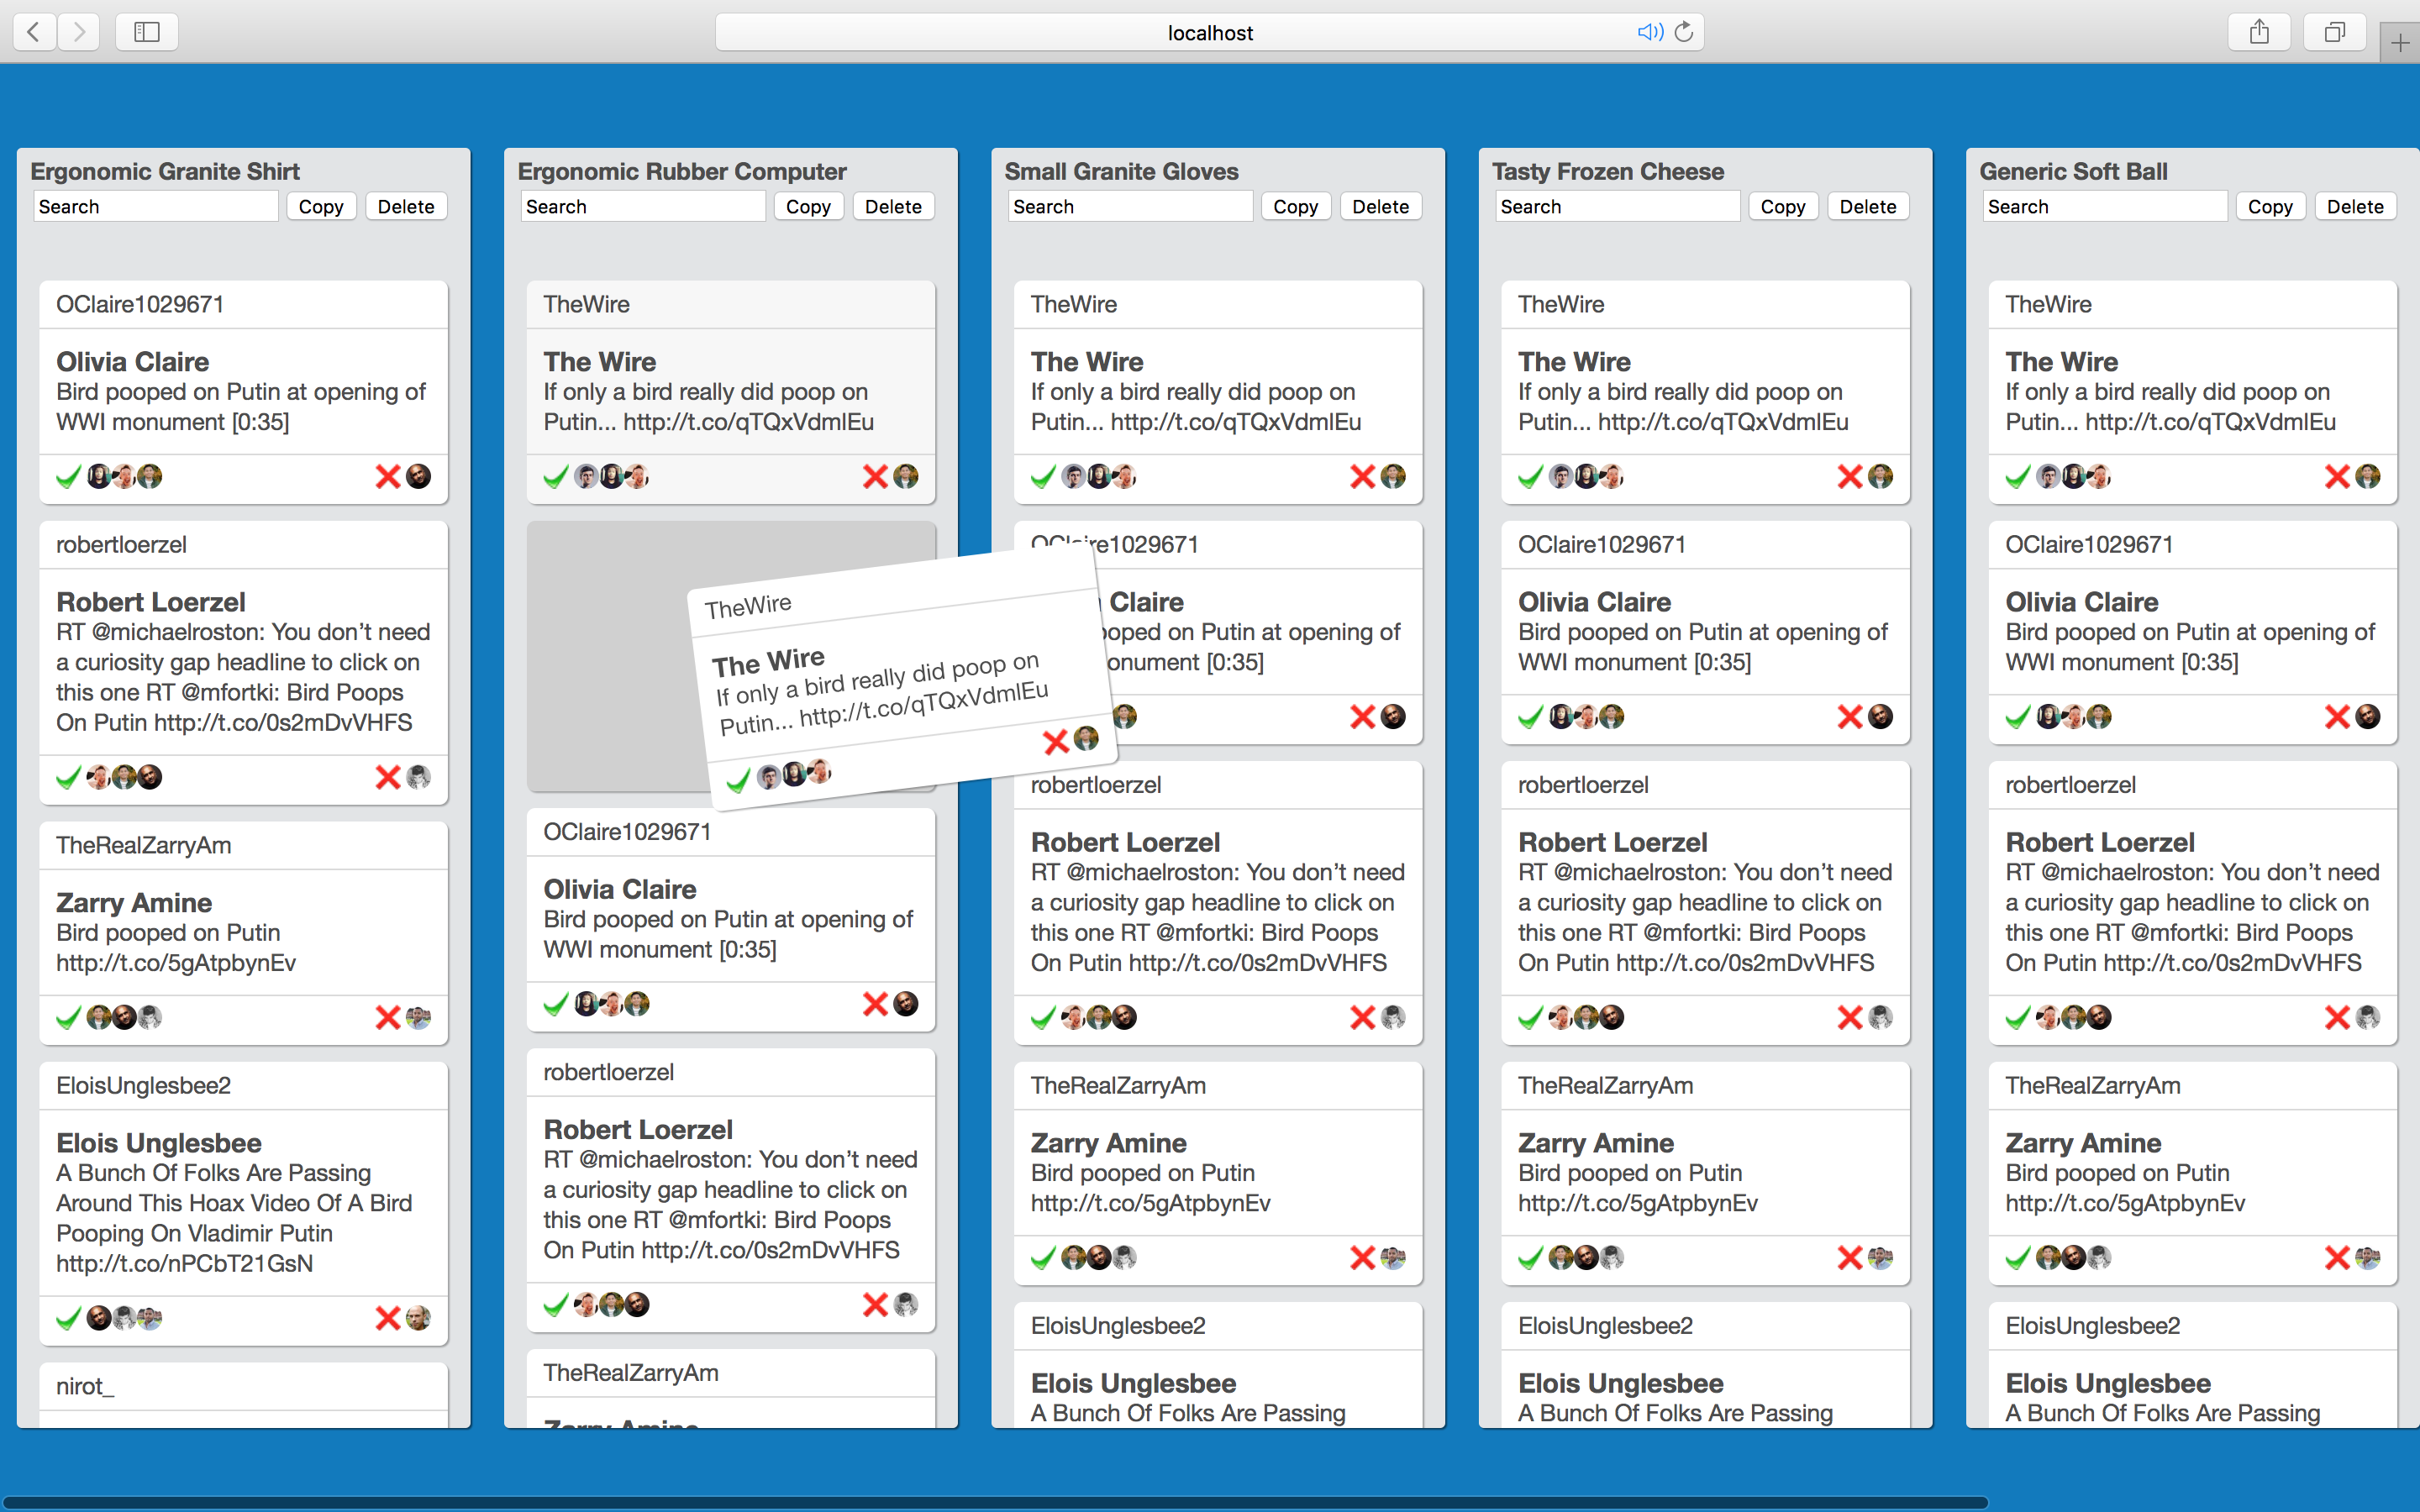
\includegraphics[width= \textwidth]{images/vector_deck}
   \caption{The UI view of vector deck for organizing tweets.  } ~\label{fig: vector_deck}
\end{figure*}


\section{General Explanation of Tweet Embedding}

\subsection{How the tweet embedding works?}


RNN更像是个动态规划
两个N个字句子之间的距离是前N-1个字,然后用各自最后一个字修改距离



RNN is more like a dynamic programming. The distance of 

rnn会对vector做incremental的修改
比如多一个字vector就变一变
变得越少意思越近






\subsection{Traditional News Discovery Process from Tweets}
Today, more and more sources of news are from social media. Newman et al. \cite{Newman2011} find that the social media is more important than mainstream media, like TV, newspapers and magazine, to play a role to broadcast news and information to general audience. Due to the large participants and diversity of information, social media could have breaking news earlier than that in mainstream media \cite{Kwak2010}. The journalists in news agency highly focus on the news feeds and resources from social media, such as Twitter, Facebook and Instagram. However, even if the journalist professionals, verifying false rumors and misinformation are still time-consuming and difficult work. In most of case, journalist professionals filter them via the information credibility \cite{Silverman2014}. 

According to the guideline in Verification Handbook \cite{Silverman2014}, amid the community and practices of journalism, journalists and reporters spend large mount of time and attention to verify news source, contacts with the relevant witnesses and build the evidence chain for the storylines. And finally make a report for the press. 

The world leading news agency developed their own process to help their journalists and reporters to verify the rumor and misinformation from social media. For example, the Associated Press (AP) created a longstanding guidance on verification, rather than to new tools and technology. In AP, the verification process of user generated content challenged the traditional new agency, andweb push them to directly contact with people to verify the information. 

At the same time, the result of our preliminary survey for the journalists in Thomson Reuters is also similar as the guideline above. Their daily process to deal with the news resource from social media includes Discover and Verify steps:

\begin{itemize}
  \item Discover Step: Most of social media journalists are using a tool, called TweetDeck, to monitor various channels in social media. It is a ``de facto" industrial standard tool for many journalists from different news agencies. 
\item Verify Step: It is same as suggested in Verification Handbook \cite{Silverman2014}: 
\begin{itemize}
  \item Find the original source; 
  \item Evaluate the credibility of the source;
  \item Try to manually verify by contacting the news source.
\end{itemize}
\end{itemize}





\section{User Interface Design}


\subsection{Hashtag }




\section{User Study}

This section will introduce the research questions we would explore and detail information about our participants, experimental setting, and the study methodology we would deploy. 

We will conduct a controlled experiment to evaluate the effectiveness of predicted hashtags and tweet embedding from RNN model for the tweets news discovery task.    

Our study would compare the TwitterDeck like app with predicted hashtags and tweet embedding from RNN model to the other normal TwitterDeck like app without RNN model support.  

In this study, we will recruit the undergraduate students from Department of Communication, Virginia Tech for this study. We suppose the participants would have experience with news discovery and news article writing with social media.

\subsection{Compared Techniques}

We will compare four different techniques in our study:

\begin{itemize}
  \item \textbf{TwitterDeck Like App (T)} is implemented with the basic keywords search and tweets drag-and-drop functions of TwitterDeck. Similar with the keywords search normally, the keywords search in this technique is to match keywords exactly in the text of tweets. This widely adopted technique will be served as a baseline condition in our study. 
  
  \item \textbf{TwitterDeck Like App with Predicted Hashtag only (H)} adds the predicted hashtag from RNN model for each tweets in TwitterDeck Like App. Users can organize tweets via the predicted hashtags in different columns. At the same time, users can also apply all the functions in the \textbf{TwitterDeck Like App (T)} above. The detail of hashtag predictions from RNN model has been introduced in Section 3. 

  \item \textbf{TwitterDeck Like App with Tweet Embedding only (E)} plugs the tweet embedding from RNN model to each tweets in TwitterDeck Like App. In this technique, users can search the keywords for the relevant tweets in vector space. In this technique, we believe users would reach more relevant tweets without exactly matching in keywords. For the detail of tweet embedding from RNN model and search in vector space model, we have discussed in Section 3.   
  
  \item \textbf{TwitterDeck Like App with both Predicted Hashtags and Tweet Embedding (H\&E)} is the combination of third \textbf{H} and fourth \textbf{E} techniques. Users would organize and search tweets with the ultimate supports from RNN model. 
  
\end{itemize}

The Figure 5 shows an user interface example of the four different techniques applied to the same tweets data. 

\subsection{Tasks and Apparatus}

Users would be asked to perform a news discovery task from tweets via user interface techniques we provided. In the typical news discovery process, social media journalists would look for 




Users were asked to perform a modified visual search task. In a con- ventional visual search task, the user looks for a specific target item within multiple distractors; a single instance of the target is usually present in about 50\% of the presented images [30]. In our experi- ment, users were required to identify multiple targets within complex images that were visually enhanced by one of the highlighting tech- niques described above. This task represents a typical visual search task of knowledge workers, who need to scan related elements in mul- tiple views or items related to their current selection in a single visual- ization. To assess whether users identified all the highlighted elements in the image, we asked them to count as accurately and quickly as possible the number of elements found. Users were instructed that accuracy was considered more important than task completion time.

Because we did not wish to limit our technique to a single sce- nario, we presented users with 16 different use case images for each technique. These images included scatterplot matrices, biochemical pathways, satellite images, and treemaps as well as multiple appli- cation windows containing text, images, and maps (Figure 10). In addition, we varied the number of highlighted elements across these images from 5 to 12, with two occurrences each.


\subsection{Design and Procedure}

\subsection{Hypotheses}

\subsection{Results}


\subsection{Research Questions}

In this paper, the goal we want to evaluate are two things:

\subsection{Predicted Hashtags By RNN}

Will the predicted hashtag can help the users to organize the tweets? How it works? Would the predicted hashtag would reduce the mental demand and physical demands of users?

Compared self-defined hashtag by users, what's the advantages of predicted hashtags and other previous techniques?


\subsection{Vector Space Search by RNN}

Will the vector space search feature can help users 

\begin{figure}[thb!]
    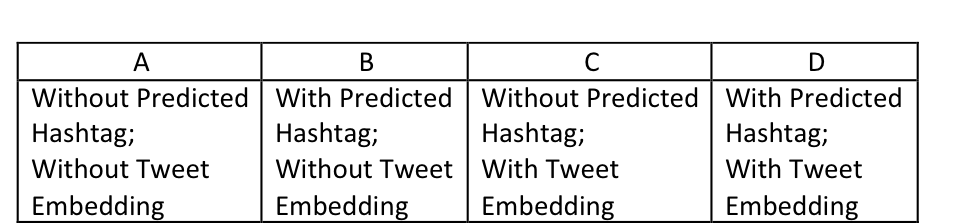
\includegraphics[width= 1.1 \columnwidth]{images/user_study_plan}
   \caption{The UI view of vector deck for organizing tweets.  } ~\label{fig: vector_deck}
\end{figure}


\subsection{Proposed Study Methodology}



\section{Evaluation Results}


\section{Contributions}

The first contribution of this paper is to use the RNN model to predict the hashtag and generate RNN based tweet embedding to support the vector space model. These two highlight spots 

We utilize recurrent neural network (RNN) to train a classification model for hashtag prediction of any texts. Our RNN model can achieve $51.86\%$ in prediction rate, which is ~2x higher than the traditional Bag-Of-Word (BOW) prediction model. Secondly, we built a RNN we designed a rumor tweets visualization system with the sentence embeddings from our RNN model. 


The second contribution is that we conducted a controlled experiment that compared the use of four different techniques to support typical tweets news discovery tasks of social media journalists: simple twitter deck like approach,  approach with predicted hashtag only, approach with tweet embedding search only,  and approach with both predicted hashtags and tweet embedding search.

We expect the results of this experiment would show that predicted hashtags and tweet embedding search from RNN model could improve performance on tasks for social media news discovery related mounts of tweets. We also expect the results would show that the approach with both predicted hashtags and tweet embedding search is the most effective of the four techniques we tested.












